\documentclass[12pt]{exam}

\usepackage{amssymb, amsmath, amsthm, mathrsfs, multicol, graphicx}
\usepackage{tikz}
 \def\d{\displaystyle}
\def\?{\reflectbox{?}}
\def\b#1{\mathbf{#1}}
\def\f#1{\mathfrak #1}
\def\c#1{\mathcal #1}
\def\s#1{\mathscr #1}
\def\r#1{\mathrm{#1}}
\def\N{\mathbb N}
\def\Z{\mathbb Z}
\def\Q{\mathbb Q}
\def\R{\mathbb R}
\def\C{\mathbb C}
\def\F{\mathbb F}
\def\A{\mathbb A}
\def\X{\mathbb X}
\def\E{\mathbb E}
\def\O{\mathbb O}
\def\U{\mathcal U}
\def\pow{\mathcal P}
\def\inv{^{-1}}
\def\nrml{\triangleleft}
\def\st{:}
\def\~{\widetilde}
\def\rem{\mathcal R}
\def\sigalg{$\sigma$-algebra }
\def\Gal{\mbox{Gal}}
\def\iff{\leftrightarrow}
\def\Iff{\Leftrightarrow}
\def\land{\wedge}
\def\And{\bigwedge}
\def\AAnd{\d\bigwedge\mkern-18mu\bigwedge}
\def\Vee{\bigvee}
\def\VVee{\d\Vee\mkern-18mu\Vee}
\def\imp{\rightarrow}
\def\Imp{\Rightarrow}
\def\Fi{\Leftarrow}

%\def\={\equiv}
\def\var{\mbox{var}}
\def\mod{\mbox{Mod}}
\def\Th{\mbox{Th}}
\def\sat{\mbox{Sat}}
\def\con{\mbox{Con}}
\def\bmodels{=\joinrel\mathrel|}
\def\iffmodels{\bmodels\models}
\def\dbland{\bigwedge \!\!\bigwedge}
\def\dom{\mbox{dom}}
\def\rng{\mbox{range}}
\DeclareMathOperator{\wgt}{wgt}


\def\bar{\overline}


\newcommand{\vtx}[2]{node[fill,circle,inner sep=0pt, minimum size=4pt,label=#1:#2]{}}
\newcommand{\va}[1]{\vtx{above}{#1}}
\newcommand{\vb}[1]{\vtx{below}{#1}}
\newcommand{\vr}[1]{\vtx{right}{#1}}
\newcommand{\vl}[1]{\vtx{left}{#1}}
\renewcommand{\v}{\vtx{above}{}}

\def\circleA{(-.5,0) circle (1)}
\def\circleAlabel{(-1.5,.6) node[above]{$A$}}
\def\circleB{(.5,0) circle (1)}
\def\circleBlabel{(1.5,.6) node[above]{$B$}}
\def\circleC{(0,-1) circle (1)}
\def\circleClabel{(.5,-2) node[right]{$C$}}
\def\twosetbox{(-2,-1.4) rectangle (2,1.4)}
\def\threesetbox{(-2.5,-2.4) rectangle (2.5,1.4)}
\newcommand{\twoline}[2]{\begin{pmatrix}#1 \\ #2 \end{pmatrix}}


\def\d{\displaystyle}
\def\?{\reflectbox{?}}
\def\inv{^{-1}}
\def\b#1{\mathbf{#1}}
\def\f#1{\mathfrak #1}
\def\c#1{\mathcal #1}
\def\s#1{\mathscr #1}
\def\r#1{\mathrm{#1}}
\def\N{\mathbb N}
\def\Z{\mathbb Z}
\def\Q{\mathbb Q}
\def\R{\mathbb R}
\def\C{\mathbb C}
\def\F{\mathbb F}
\def\A{\mathbb A}
\def\X{\mathbb X}
\def\E{\mathbb E}
\def\O{\mathbb O}
\def\FR{\mathscr{F(\R)}}
\def\pow{\mathscr P}
\def\inv{^{-1}}
\def\nrml{\triangleleft}
\def\st{:}
\def\~{\widetilde}
\def\rem{\mathcal R}
\def\iff{\leftrightarrow}
\def\Iff{\Leftrightarrow}
\def\and{\wedge}
\def\And{\bigwedge}
\def\AAnd{\d\bigwedge\mkern-18mu\bigwedge}
\def\Vee{\bigvee}
\def\VVee{\d\Vee\mkern-18mu\Vee}
\def\imp{\rightarrow}
\def\Imp{\Rightarrow}
\def\Fi{\Leftarrow}


\def\dom{\mbox{dom}}
\def\rng{\mbox{range}}



\def\bar{\overline}

%\pointname{pts}
\pointsinmargin
\marginpointname{pts}
\marginbonuspointname{ bns pts}

\addpoints
\pagestyle{headandfoot}
\printanswers

\firstpageheader{Math 228}{\bf\large Exam 1 -- Take Home\\Solutions}{Fall 2018}
\runningfooter{}{\thepage}{}
\extrafootheight{-.45in}



\begin{document}
%space for name
% \noindent {\large\bf Name:} \underline{\hspace{2.5in}}
% \vskip 1em
%
% \noindent{\bf Instructions:} This is the take-home portion of the first exam.  Here are my expectations:
%
% \begin{itemize}
% \item WORK ALONE!  You may \underline{not} collaborate or discuss problems with other students, either in or outside of this class.  Also do not discuss with tutors, significant others, parents, kids, etc.  Cats and dogs are okay, but only if they have not taken discrete math class. If you need clarification on a problem, ask me.
%
% \item You may use your notes and the textbook, but only notes you have taken in this class and only the assigned textbook from this class.  This is intended only for you to refresh your memory if you forget a definition, not for you to copy proofs (or even the style of proof) from your notes.  Alternatively, if you do not remember a definition, send me an email.
%
% \item Other than your notes and textbook, do not use any outside sources. In particular, absolutely NO INTERNET.
%
% \item This is not a timed exam, and you may take as much time on it as you like.  However, I do not intend for you to spend more than 2 hours total working on the exam.
%
% \item You should write up all solutions neatly on your own paper and staple this sheet to your solutions, and sign below.  Clearly number each problem.  Preferably, use one sheet of paper per problem, and leave lots of room around your work.
%
% \item As always, you must show all your work to receive credit, and explanations and proofs should be written out in complete English sentences.  A page of just equations and calculations will probably receive no credit.
%
% \item \textbf{Due Monday, October 1.}
% \end{itemize}
%
% \centerline{Have Fun!}
%
%
% \vfill
%
% \begin{center}
% 	\emph{By signing below, I certify that the work on this take-home exam is solely my own, that I did not receive assistance from anyone other than my instructor, and did not use resources other than my own notes and the course textbook.}
%
% \end{center}
% \vskip 1em
% \noindent {\large Signature:} \underline{\hspace{3in}} \hspace{2em} {\large Date:} \underline{\hspace{1.5in}}
%
%
%
% \vskip 1em
%
% % \hrulefill
% % \vskip 2em
% \clearpage

\begin{questions}
\question[10] Give an example of an implication (i.e., if-then statement) about graphs which is true, but that has a false converse.  Write both the original implication and converse, and then explain how you know the converse really is false.

\begin{solution}
	There are many examples here.  For example:
	\begin{itemize}
		\item If a graph is planar, then it's chromatic number is 4.  The converse (if a graph has chromatic number 4, then it is planar) is false, as seen in $K_{3,3}$.
		\item If a graph is a tree, then $v = e+1$.  The converse (if a graph has $v = e+1$, then it is a tree) is false, which you can see by looking at a disconnected graph.
		\item If a graph has an Euler cycle, then it is connected.  The converse (if a graph is connected, then it has an Euler cycle) is false, as seen by a tree, for example.
	\end{itemize}
\end{solution}

\question[20] Consider the statement, ``If a graph $G$ has $n$ vertices and every vertex is adjacent to every other vertex in the graph, then $G$ has $\frac{n(n-1)}{2}$ edges.''
\begin{parts}
	\part Prove this statement is true using a direct proof, proof by contrapositive, or proof by contradiction.  Indicate what style of proof you are using.
	\begin{solution}
		We will give a direct proof.  Suppose $G$ has $n$ vertices and that every vertex is adjacent to every other vertex.  Then each vertex will have degree $n-1$, so the sum of the degrees will be $n(n-1)$.  However, this counts every edge exactly twice, so there are $\frac{n(n-1)}{2}$ edges.
	\end{solution}
	\part Give a second careful proof of this statement, this time using mathematical induction.  Make sure your proof is formatted correctly.
	\begin{solution}
		Let $P(n)$ be the statement, ``For all graphs $G$ with $n$ vertices, if every vertex is adjacent to every other vertex, then $G$ has $\frac{n(n-1)}{2}$ edges.''

		Base case: If $n = 1$, there are zero edges (there is only one graph with one vertex).  Indeed, $1(1-0)/2 = 0$.

		Inductive case.  Fix $k\ge 1$ and assume $P(k)$ is true.  Now consider an arbitrary graph $G$ with $k+1$ vertices and assume that all vertices are adjacent to all other vertices in $G$.  Let $v$ be any vertex and consider the graph $G'$ you get by removing $v$ and its $k$ edges.  This graph $G'$ has $k$ vertices, all adjacent, so by the assumption of $P(k)$ we see that $G'$ has $\frac{k(k-1)}{2}$ edges.  Now looking back at $G$, we have a graph with $k$ more edges than $G'$.
		But $\frac{k(k-1)}{2} + k = \frac{k(k-1)+2k}{2} = \frac{(k+1)k}{2}$, so $G$ has $\frac{(k+1)k}{2}$ edges, which is what $P(k+1)$ requires.

		Therefore, by the principle of mathematical induction, $P(n)$ is true for all $n \ge 1$.
	\end{solution}
\end{parts}

\question[10] Suppose $G$ is a graph with an Euler cycle.  Let $G'$ be a graph isomorphic to $G$.  Must every vertex in $G'$ have even degree?  Prove your answer.

\begin{solution}
	Yes.  Suppose $G$ has an Euler cycle and that $G'$ is isomorphic to $G$.  Since $G$ has an Euler cycle, we know that every vertex of $G$ must have even degree.  Since the degree sequence of a graph is preserved under isomorphism, we see that $G'$ must then also have all its vertices have even degree.
\end{solution}

\question[10] Consider the graph drawn below.  Find the chromatic number of the graph and carefully prove that your answer is correct (i.e., prove that the chromatic number cannot be more or less than what you say it is).

\begin{center}
	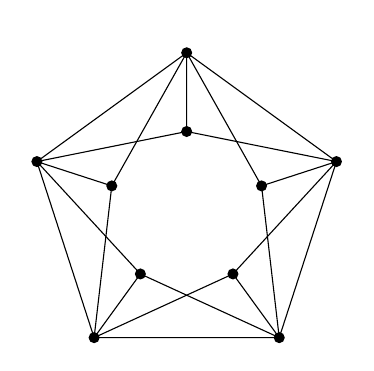
\begin{tikzpicture}
		\foreach \x in {0,...,4}{
		\draw (90+\x*72:1) -- (90+\x*72:2) -- (162+\x*72:2) -- cycle -- (18+\x*72:2);
		\draw (90+\x*72:1) \v (90+\x*72:2) \v;
		}
	\end{tikzpicture}
\end{center}

\begin{solution}
	It is fairly easy to give a 4-coloring of the graph (use three colors on the outside cycle and a 4th for the five inside vertices).  This proves that the chromatic number cannot be more than 4.

	To see that the chromatic number cannot be less than 4, suppose that there is a proper 3-coloring.  Then these three colors must all be used on the outside $C_5$.  In fact, two colors must be used twice (say red and blue) and the third color must be used once (say green).  It must be the case that the green vertex is adjacent to one red and one blue vertex in the copy of $C_5$.  But then these three vertices are also adjacent to one ``inside'' vertex, which cannot be colored.  This contradiction proves that 4 colors are required.
\end{solution}

\bonusquestion[10] Bonus!! Before you sit three chests -- one made of wood, one of stone, and one of steel.  You know that one of the chests contains a great treasure, while the other two contain vicious, angry, man-eating, deadly poisonous scorpions (also known as {\em scorpions}).

On each chest hangs a sign, giving you information about which chest contains the treasure.  Problem is, you do not know which signs are true and which are false.  The signs read:
\begin{itemize}
  \item[Wood chest:] If the sign on the stone chest is true, then the treasure is not in the steel chest.
  \item[Stone chest:] Exactly two of these signs are false. % and the treasure is not in this chest.
  \item[Steel chest:] The treasure is in a chest with a false sign.
\end{itemize}
Which chest contains the treasure?  Prove your answer is correct.

(For some partial credit, determine the truth or falsity of one or more signs and explain.)

\begin{solution}
 The treasure is in the stone chest.

 \begin{proof}
  Consider the stone chest's sign.  If the sign were true, then both of the other signs would be false.  However, the wood chest's sign being false means that the sign on the stone chest is true {\em and} the treasure {\em is} in the steel chest.  So the treasure would be in the steel chest, a chest with a false sign, making the steel chest's sign true.  This is a contradiction.  Therefore the stone chest's sign must be false.

  Now we know that either all three signs are false or just the stone chest's sign is false (if one other sign was false, that would be two false signs, which we know is not the case).  However, it cannot be that all three signs are false: if the wood chest's sign is false, that means the stone chest's sign is true, a possibility we have already discounted.  Therefore the signs on both the wood and steel chests are true.  In particular, it is true that the treasure is in a chest with a false sign.  There is only one such chest: the stone chest, wherein lies the treasure.
 \end{proof}

\end{solution}
\end{questions}




\end{document}
